\chapter{Iteración 1: “Elección de la solución”}
    \begin{section}{Security Onion como sistema de gestión de eventos}
    \begin{figure}[H]
        \centering
        
\includegraphics[width=0.7\textwidth]{./iteracion_1_imagenes/figura_15_logo_sonion.png}
        \caption{logo de Security Onion\cite{sonion}}
        \label{fig:logo_sonion}
    \end{figure}
        La elección de Security Onion como plataforma se justificó en su naturaleza de código abierto y por sus características destacables respecto de otras soluciones libres, como el soporte de una activa comunidad, el desarrollo continuo de mejoras, actualizaciones y correcciones, su capacidad polimórfica y funcional de actuar como IDS, plataforma SIEM o cluster de almacenamiento. Esto permitió desarrollar distintas arquitecturas de una manera fácil y asistida para el despliegue y la consiguiente optimización de los recursos de hardware y de red. \par
        Otras de las propiedades destacables es la capacidad de integración directa con un conjunto casi universal de los sistemas IDS disponibles, tanto libres como propietarios. Security Onion también incluye un paquete de configuraciones iniciales predefinidas para la infraestructura inicial del sistema, tales como el almacenamiento, normalización y gestión de logs (pila Elastic),  los sistemas IDS y de gestión de usuarios, entre otros. \par
    \end{section}
    \begin{section}{Arquitectura del sistema de gestión de eventos}
    \end{section}
    \begin{subsection}{Arquitectura de alto nivel}
    \begin{figure}[H]
        \centering
        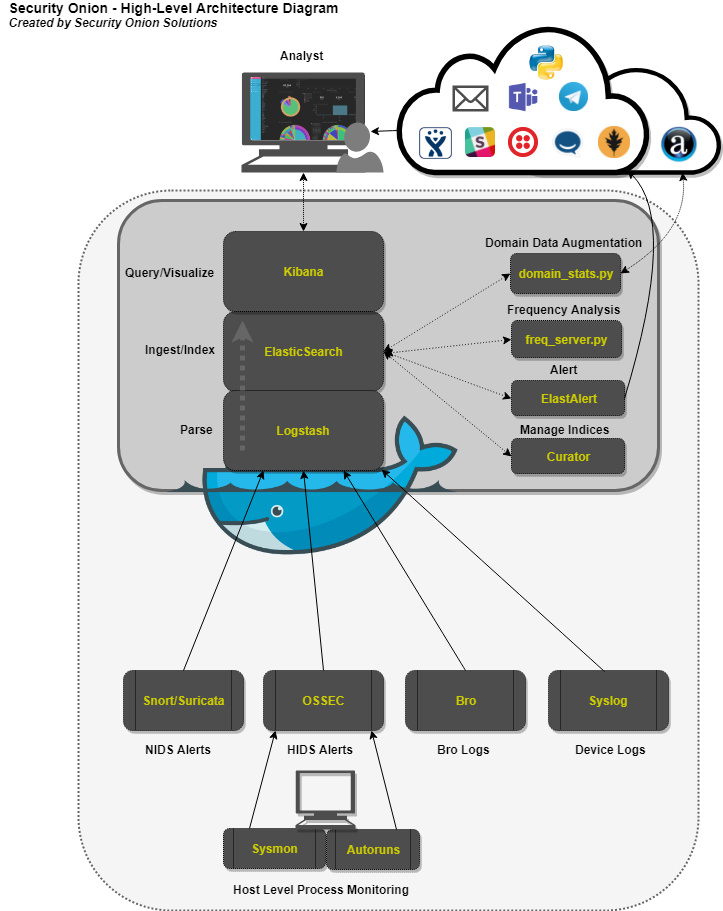
\includegraphics[width=0.7\textwidth]{./iteracion_1_imagenes/figura_16_arq_alto_nivel_sonion.png}
        \caption{Security Onion\cite{sonion}: Arquitectura de alto nivel}
        \label{fig:arq_top_sonion}
    \end{figure}
    En la Figura \ref{fig:arq_top_sonion} se observa la distribución de Security Onion y el flujo de datos entre sus componentes principales (la pila Elastic) y secundarios (Curator \cite{curator}, ElastAlert\cite{elasalert}, freqServer\cite{freqserver} y domainStats\cite{domainstat}). Se puede apreciar la conexión con los sistemas de detección IDS como Bro\cite{zeek}, Snort\cite{snort}, Suricata\cite{suricata}, Syslog, etc. Se distinguen también los enlaces con los puntos de administración de los analistas del CSIRT y con los servicios web externos para el envío y recepción de alertas, notificaciones, análisis de tráfico, entre otros. Un punto a destacar es que la pila Elastic se encuentra desplegada en contenedores Docker\cite{docker}. 
    \end{subsection}
    \pagebreak
    \begin{subsubsection}{Tipo de Nodos}
        \begin{itemize}
          \item Nodo Master: este nodo ejecuta su propia copia de la base de datos Elasticsearch, con la que gestiona las búsquedas a través del cluster y estructura a otros nodos en el momento de su despliegue. Lo anterior implica que puede realizar las configuraciones necesarias para los nodos de los tipos “densos” y los de almacenamiento, pero no los de sensores o Forward, por carecer estos últimos de una pila Elastic. Este nodo permite a un analista conectarse mediante un enlace de supervisión para realizar consultas de los datos.
          \begin{itemize}
              \item  Este nodo contiene los siguientes componentes:
              \begin{itemize}
                  \item Elasticsearch \cite{elastic}
                  \item Logstash \cite{elastic}
                  \item Kibana \cite{elastic}
                  \item Curator \cite{curator}
                  \item ElastAlert \cite{elasalert}
                  \item Redis \cite{redis}
                  \item Wazuh \cite{wazuh} / OSSEC \cite{ossec}
                  \item Sguild \cite{sguil}
              \end{itemize}
          \end{itemize}
          Elasticsearch \cite{elastic}, Kibana \cite{elastic} y Logstash \cite{elastic} son componentes de la pila Elastic, que se tratarán en la siguiente sección junto a ElastAlert \cite{elasalert}. El objetivo de Curator \cite{curator} y Redis \cite{redis} es administrar y optimizar las bases de datos de los nodos de almacenamiento; Wazuh \cite{wazuh} es un IDS y Security Onion lo utiliza para el monitoreo de sí mismo, configurando un sistema HIDS ad hoc, aunque es posible desplegarlo en otros nodos o puntos de interés. Sguild \cite{sguil} permite consultar eventos de una base de datos MySQL desde dentro de Security Onion y muestra los resultados en una GUI. Además, actúa como intermediario de otros componentes secundarios como Squert \cite{squert}, del que detallaremos sus funciones y comportamiento en una sección posterior. 
          \item Nodos Forward: este nodo cumple la función de procesar el tráfico y reenviar los resultados al nodo master. Los logs generados por Snort / Suricata y Bro son enviados mediante syslog a Logstash en el nodo master, utilizando un túnel ssh, donde finalmente son guardados en la base de datos Elasticsearch, donde pueden ser reenviados a los nodos de almacenamiento. Los logs pueden ser consultados a través de una búsqueda en el cluster
            \begin{itemize}
               \item Los componentes de un nodo Forward son:
               \begin{itemize}
                   \item Zeek \cite{zeek} (sucesor de Bro)
                   \item Snort \cite{snort} / Suricata \cite{suricata}
                   \item Netsniff-ng \cite{netsniff-ng}
                   \item Wazuh \cite{wazuh} / OSSEC \cite{ossec}
                   \item Syslog-ng \cite{syslog-ng}
               \end{itemize}
            \end{itemize}
            Zeek, Snort / Suricata y Netsniff-ng son procesadores de tráfico (IDS), donde Snort y Suricata serán tratados en una sección posterior. Syslog-ng es utilizado para recolectar logs de los IDS y enviarlos al Logstash del master, donde serán procesados y tratados antes de ser escritos en Elasticsearch.
            \item Nodos Pesados: Es un nodo híbrido entre el nodo Forward y el nodo Master, que incluye todos los componentes del nodo Forward, además de una instancia completa de la pila Elastic. Los nodos pesados envían los resultados de las consultas de su instancia local de Elasticsearch a las solicitudes realizadas por el nodo master mediante un túnel de autossh.
            \begin{itemize}
                \item Los componentes de este nodo son:
                \begin{itemize}
                    \item Elasticsearch
                    \item Logstash
                    \item Curator
                    \item Zeek
                    \item Snort / Suricata
                    \item Netsniff-ng
                    \item Wazuh / OSSEC
                    \item Syslog-ng (envía los logs a la instancia local de Logstash)
                \end{itemize}
            \end{itemize}
            \item Nodos de almacenamiento: su objetivo es extender las capacidades de almacenamiento y procesamiento del nodo master. Estos nodos despliegan una instancia local de la pila Elastic. De manera análoga a los nodos pesados, cuando se realiza una consulta por parte de la instancia Elasticsearch del nodo master, esta es procesada por la instancia local del nodo de almacenamiento y devuelta por un túnel autossh.
            \begin{itemize}
                \item Los componentes del nodo de almacenamiento son:
                \begin{itemize}
                    \item Elasticsearch
                    \item Logstash
                    \item Curator
                    \item Wazuh / OSSEC
                \end{itemize}
            \end{itemize}
        \end{itemize}
    \end{subsubsection}
    \pagebreak
    \begin{subsubsection}{Tipos de Arquitectura}
      La versatilidad de disponer de múltiples arquitecturas permite adaptar la plataforma a las necesidades de la organización en la que se implante. A continuación, se describen cada una de las opciones posibles:
    \begin{itemize}
         \item Arquitectura monolítica: Consiste en un único servidor que ejecuta simultáneamente los componentes centrales o propios de un nodo master y los de un nodo sensor. Es un modo híbrido y concentrado que no se recomienda para enlaces de red de alto rendimiento por los elevados requerimientos de hardware necesarios. 
         Este tipo de arquitectura se recomienda para propósitos de pruebas en laboratorio y en entornos de baja demanda de tráfico de red.
        \begin{figure}[H]
            \centering
            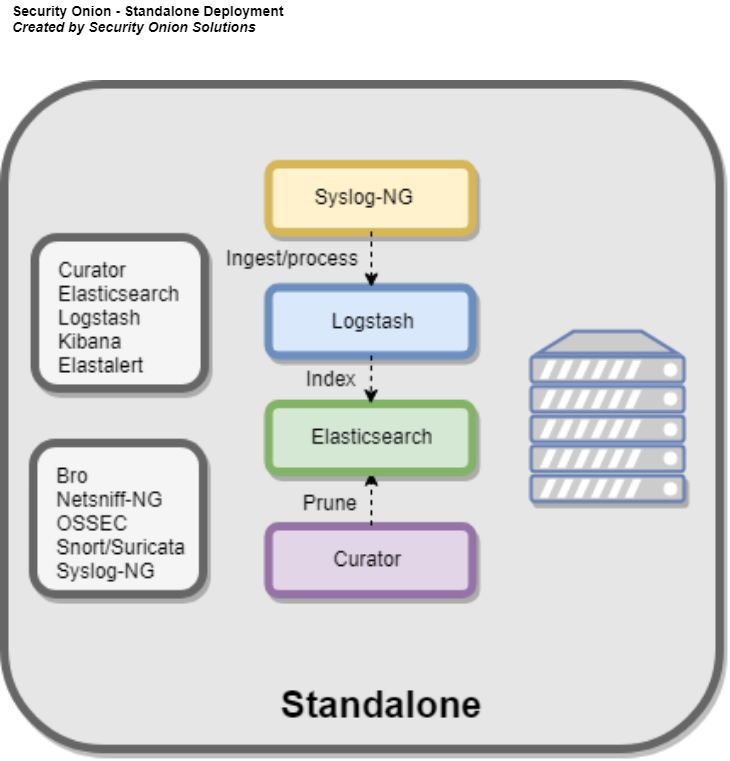
\includegraphics[width=0.7\textwidth]{./iteracion_1_imagenes/figura_17_arq_monolitica_sonion.png}
            \caption{Arquitectura monolítica de Security Onion\cite{sonion}}
            \label{fig:arq_monolitica_sonion}
        \end{figure}
        \FloatBarrier
        \pagebreak
        \item Arquitectura densamente distribuida: consiste en uno o más nodos pesados conectados a un nodo master. Solo se recomienda en el caso de que no sea posible desplegar una arquitectura distribuida, ya que tiene las mismas deficiencias de rendimiento de la arquitectura monolítica y no es apropiado para entornos de producción y/o enlaces de red de alta velocidad.
        \begin{figure}[H]
            \centering
            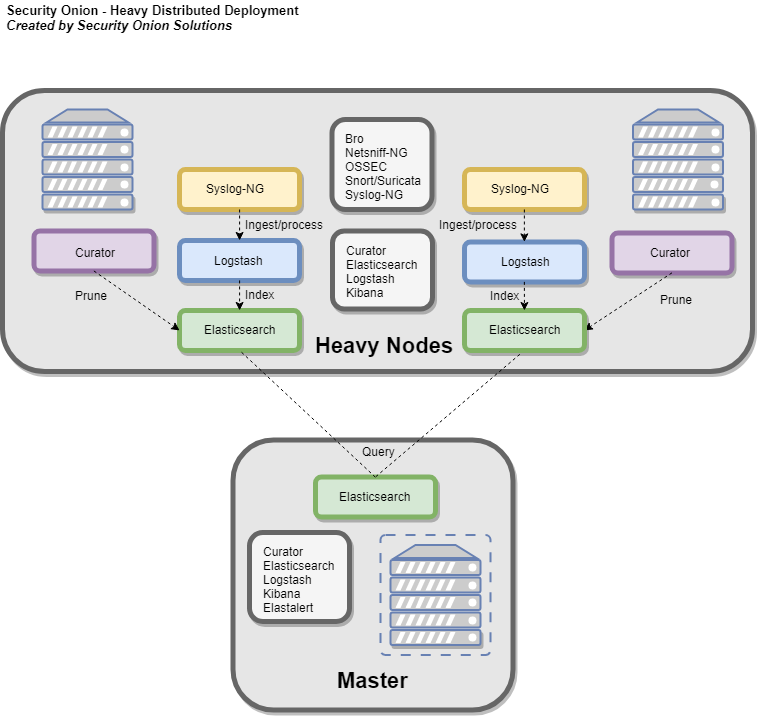
\includegraphics[width=0.7\textwidth]{./iteracion_1_imagenes/figura_18_arq_densa_sonion.png}
            \caption{Arquitectura densamente distribuida de Security Onion\cite{sonion}}
            \label{fig:arq_densa_sonion}
        \end{figure}
        \FloatBarrier
        \pagebreak
        \item Arquitectura Distribuida: consiste en un servidor master, uno o más nodos Forward y uno o más nodos de almacenamiento. Es el tipo de despliegue recomendado en términos de eficiencia de requerimientos de hardware, balance de la carga y almacenamiento de datos y optimización general de los recursos disponibles en la organización. 
        \begin{figure}[H]
            \centering
            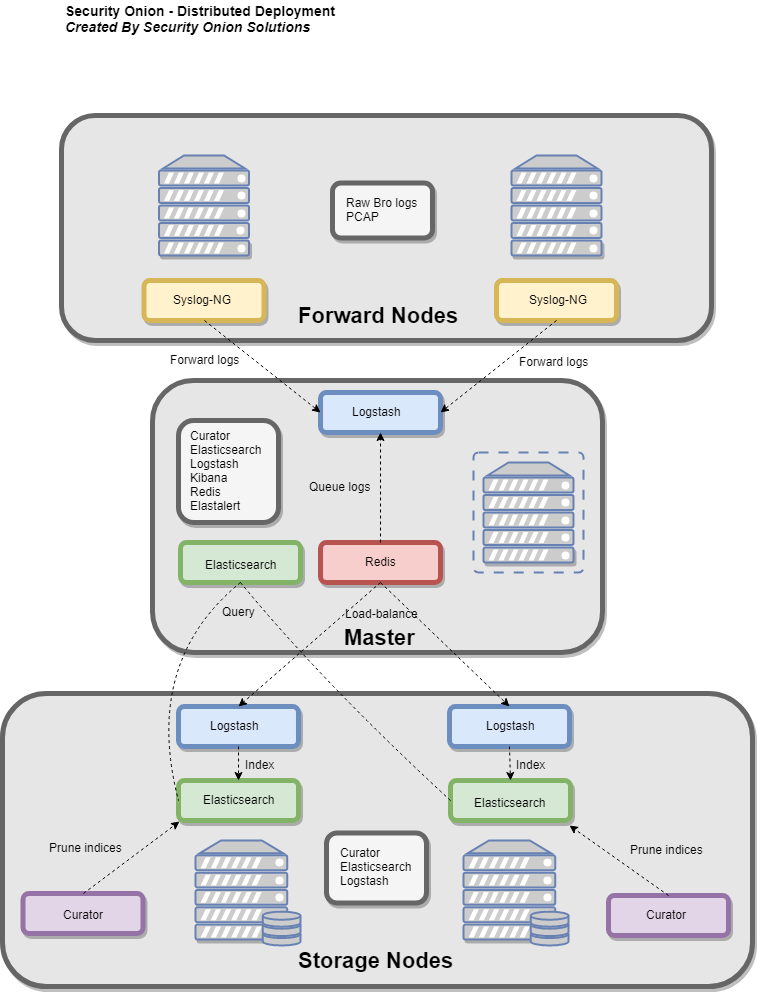
\includegraphics[width=0.7\textwidth]{./iteracion_1_imagenes/figura_19_arq_distribuida_sonion.png}
            \caption{Arquitectura distribuida de Security Onion\cite{sonion}}
            \label{fig:arq_distribuida_sonion}
        \end{figure}
     \end{itemize}
   \end{subsubsection}
   \pagebreak
   
   \begin{section}{Arquitectura del despliegue }
    \begin{figure}[H]
        \centering
        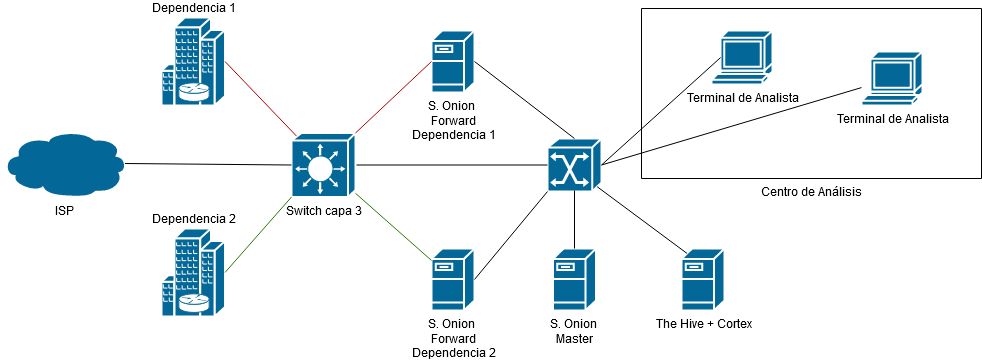
\includegraphics[width=1\textwidth]{./iteracion_1_imagenes/figura_33_arquitectura_despliegue_proyecto.png}
        \caption{Arquitectura de Despliegue}
        \label{fig:arquitectura_despliegue_proyecto}
    \end{figure}
    \FloatBarrier
    En la Figura \ref{fig:arquitectura_despliegue_proyecto} se muestra la arquitectura de despliegue del proyecto. La descripción, de izquierda a derecha, es: el proveedor ISP de conexión a internet y por consiguiente al exterior de la organización, el switch de capa 3 al que están conectadas las dependencias cuyos enlaces fueron seleccionados para ser monitoreados para este proyecto, los nodos Forward de Security Onion y un switch de la red interna del CSIRT. Se observa que los enlaces “Dependencia 1 - switch capa 3” y el de “switch capa 3 - nodo Forward de Security Onion Dependencia 1” tienen el mismo color; esto se debe a motivos de representar el hecho de que el switch capa 3 fue configurado para reenviar el tráfico entre el enlace de este y la dependencia 1 hacia el nodo Forward mencionado. Una situación análoga ocurre entre la Dependencia 2 y el nodo Security Onion Forward Dependencia 2. \par
    El último eslabón de la conexión, el switch de capa 2, es el encargado de la red interna del CSIRT. A él se encuentran conectados las computadoras de los analistas y el nodo Master de Security Onion, los nodos Forward anteriormente mencionados y el servidor que aloja a TheHive y Cortex. Finalmente, los analistas pueden consultar y administrar los servidores correspondientes a los nodos Master y Forward de Security Onion así como al servidor que contiene a TheHive y Cortex. \par

   \end{section}